\section{Diffusion models}\label{diffusion Models}

The limitations of VAEs and GANs, which were just stated above, have led to the emergence of diffusion models, a method that offer distinct advantages over traditional generative models. Diffusion models operate by progressively perturbing data with noise and then learning to reverse this process to generate new samples. 

~\cite{yangdiffusionSummary} distingueshe between three main approaches that dominate the study of diffusion models, which are going to be discussed shortly: Denoising Diffusion Probabilistic Models (DDPMs) \citep{hoDDPMs,sohlDDPM}, Score-based Generative Models (SGMs) \citep{song2019SGM}, and Stochastic Differential Equations (Score SDEs) \citep{song2020score, song2021maximum}.

\subsection{Denoising Diffusion Probabilistic Models}
DDPMs employ two Markov chains, a forward chain and a reverse chain, also known as the forward and reverse diffusion processes, seen in Figure~\ref{fig:figureForwardProcess} and Figure~\ref{fig:figureReverseProcess} \citep{sohlDDPM}. 

The forward diffusion process is comparable to latent variable models, sharing some similarities with Variational Autoencoders (VAEs), as focus is lying on a latent feature space of the initial data distribution. They differ in the fact that the forward process in DDPMs ``is fixed to a Markov chain that gradually [over a span of T steps] adds Gaussian noise to the data according to a variance schedule \(\beta_1, \ldots, \beta_T \)''~\cite{hoDDPMs}. This iterative process continues to add noise ``until all structures are lost'' \citep{yangdiffusionSummary} resulting in an image of pure noise. The introduction of noise aims to gradually steer the data distribution towards a more manageable prior distribution \citep{yangdiffusionSummary, pooleDreamfusion}. Mathematically, the forward process can be described in two equations:

\[
q(x_t | x_{t-1}) = \mathcal{N}(x_t; \sqrt{1 - \beta_t}x_{t-1}, \beta_t I) \quad \text{where} \quad \sqrt{1 - \beta_t}x_{t-1} = \mu_t \quad \text{and} \quad \beta_t I = \Sigma_t
\] 

\citep{martinez2023understanding}. This describes the process of adding noise to transform a data point \( x_{t-1} \) into a new data point \( x_t \). This transformation is probabilistic and follows a Gaussian distribution \citep{sohlDDPM, hoDDPMs}. The mean value of this distribution is slightly adjusted compared to the previous data point by the factor \( \sqrt{1 - \beta_t} \), which essentially corresponds to the data point \( x_{t-1} \) with a certain noise reduction. The parameter \( \beta_t \) controls the amount of noise added, where a larger \( \beta_t \) means more noise \citep{kingma2023variationalDM}. The covariance matrix, denoted \( \beta_t I \), implies that each element of the data is independently modified with the same amount of noise, since \(I\) represents an identity matrix where all outer diagonal elements are zero \citep{croitoru2023diffusion}.

\[q(x_{1:T} | x_0) = \prod_{t=1}^T q(x_t | x_{t-1}) \] 

\citep{martinez2023understanding}. In the second equation, the focus is on the entire sequence of data points from the original \( x_0 \) to \( x_T \), including all intermediate points \citep{martinez2023understanding}. This expresses the idea that to understand the probability of the entire noisy trajectory, one can calculate the probability of each step from \( x_{t-1} \) to \( x_t \) and then multiply these probabilities together. This is due to the Markov property, which states that each step is only dependent on the immediately preceding step \citep{martinez2023understanding}. This enables a comprehensive view of the transition probabilities over the entire process of noise induction, step by step.

\begin{figure}[ht]
\centering
  \includegraphics[width=1\columnwidth]{figures/manta_DDMP3.png}
  \caption{Forward process adding noise to an image}\label{fig:figureForwardProcess}
\end{figure}

The reverse chain is trained to approximate the inverse of the forward process using a deep neural network parameterized with~\(\Theta\), effectively removing the noise added by the forward chain \citep{sohlDDPM, yangdiffusionSummary}. The function \( p_\theta(x_{t-1} | x_t) \) is a probability distribution that estimates how to reverse the diffusion process. Given a data point \( x_t \), it attempts to predict the previous data point \( x_{t-1} \) before noise was added. It is modeled as a normal distribution with a mean \( \mu_\theta(x_t, t) \) and covariance \( \Sigma_\theta(x_t, t) \), both of which are functions parameterized by \( \theta \) \citep{yangdiffusionSummary}.

\[
  p_\theta(x_{t-1} | x_t) = \mathcal{N}(x_{t-1}; \mu_\theta(x_t, t), \Sigma_\theta(x_t, t))
\] 

\[p_\theta(x_{0:T}) = p_\theta(x_{T}) \prod_{t=1}^T p_\theta(x_{t-1} | x_t) \]

\citep{martinez2023understanding}. The latter function \( p_\theta(x_{0:T}) \) represents the probability of the entire sequence of data points from \( x_0 \) through \( x_T \) under the reverse process modeled by the neural network. It starts with an estimate of the final data point \( p_\theta(x_{T}) \) and works backwards through the sequence, multiplying the conditional probabilities \( p_\theta(x_{t-1} | x_t) \) for each step \citep{hoDDPMs,martinez2023understanding}. This function essentially provides a framework for reconstructing the original data from the noisy data by successively removing noise at each step, based on the learned parameters \( \theta \) \citep{yangdiffusionSummary}.


\begin{figure}[ht]
  \centering
    \includegraphics[width=1\columnwidth]{figures/manta_DDMP3.png}
    \caption{Forward process adding noise to an image}\label{fig:figureReverseProcess}
\end{figure}


The incremental introduction of the forward and backward diffusion processes offers an advantage as ``estimating small perturbations is more tractable than explicitly describing the full distribution with a single, non-analytically-normalizable, potential function'' \citep{sohlDDPM}.
According to \citep{hoDDPMs}, the neural network in the reverse process can be trained to predict one of three possibilities: the mean value of the noise at each time step, the original image itself, or the noise of the image \citep{hoDDPMs}. As previously mentioned, the second approach is not as advantageous. Hence, the research focuses on the first and last possibilities, which are essentially identical but parameterized differently. Predicting the image noise allows for straightforward subtraction of the noise from the image, resulting in a less noisy version. By employing this method iteratively, it becomes possible to completely learn an image from noise.

Nevertheless, DDPMs also have their drawbacks with the most severe being the time requirement to generate new samples \citep{xiao2022tackling}. ``This is caused by the fact that a Markov process has to be simulated at each generation step, which greatly slows down the process'' \citep{martinez2023understanding}. 

\subsection{Score-Based Generative Models}

SGMs \citep{song2019SGM} take a unique approach to generative modeling by prioritizing the learning of a score function that plays a central role in guiding the generative process. This function aims to capture the Stein score \citep{steinScore}, which is essentially ``the gradient of the log-density function at the input data point'' \citep{song2019SGM}. The score can be viewed as a vector field that indicates the direction that increases the data density the most \citep{song2019SGM}. This reveals how slight adjustments within the data can affect the overall distribution, informing the model on how to proceed with sample generation in a way that matches the actual data structure.

To train a neural network for SGMs,~\cite{song2019SGM} employ two techniques, namely Score matching and Langevin dynamics \citep{hyvarinenScoreMatching}. 
Score matching allows to train a neural network, referred to as a score network \( s_\theta(x) \), to predict the gradient of the logarithm of the probability density of the data \( \nabla_x \log p_{\text{data}}(x) \) directly without the need to first construct a model that can estimate the probability density \( p_{\text{data}}(x) \) itself \citep{song2019SGM}. The aim of this process is to minimize the difference between the predictions of the score network and the true gradient of the log-likelihood, which under certain conditions ensures that the trained network approximates the true score ``almost surely'' \citep{song2019SGM}. The term \( \frac{1}{2} \|s_\theta(x)\|^2_2 \) is part of the objective function that needs to be minimized and is used to regularize the scores predicted by the neural network while the term \( tr(\nabla_x s_\theta(x)) \), involving the trace of the Jacobian \citep{song2019SGM} of the score function, further refines the objective function by capturing the divergence of the score vector field. 

\[
\mathbb{E}_{p_{\text{data}}(x)} \left[ \text{tr}(\nabla_x s_\theta(x)) + \frac{1}{2} \|s_\theta(x)\|^2_2 \right]
\]

\citep{song2019SGM} However, scaling score matching to deep networks and high-dimensional data can be challenging due to the high computational effort required to compute certain matrix operations (such as the trace of the Jacobian matrix) \citep{song2019SGM}. 
Denoising score matching and Sliced score matching could overcome these scalability issues for large applications \citep{song2019SGM}.

In order to generate Samples, Langevin dynamics \citep{robertsLangevin} is utilized for sampling from a probability distribution by employing the score function, \( \nabla_x \log p(x) \) \citep{song2019SGM}. The process begins with an initial guess \( \tilde{x}_0 \) from a prior distribution \( \pi(x) \), and iteratively updates this guess according to the rule:

\[ \tilde{x}_t = \tilde{x}_{t-1} + \frac{\epsilon}{2} \nabla_x \log p(\tilde{x}_{t-1}) + \sqrt{\epsilon} z_t, \]

\citep{song2019SGM} where \( z_t \) follows a standard normal distribution and \( \epsilon \) is a small step size. Theoretically, as \( \epsilon \) approaches zero and the number of iterations \( T \) becomes very large, the distribution of \( \tilde{x}_T \) will converge to \( p(x) \) \citep{song2019SGM}. The score network \( s_\theta(x) \) is trained to closely estimate \( \nabla_x \log p_{\text{data}}(x) \), thus allowing for the generation of new samples that approximate the desired data distribution through Langevin dynamics \citep{song2019SGM}.

In the specific context of score-based generative modeling, there's a notable challenge to overcome. The estimated score function may not be entirely accurate in regions of the data space where there's minimal or no training data available \citep{song2019SGM}. In such cases, Langevin Dynamics might not converge correctly, resulting in complications during the sample generation process. To address this issue,~\cite{song2019SGM} suggest ``to perturb the data with random Gaussian noise of various magnitudes'', while simultaneously estimate the score functions for these noise-altered data distributions. This approach is called Noise Conditional Score Networks (NCSNs) and ensures that the resulting data distribution doesn't condense into a lower-dimensional structure \citep{song2019SGM}.

\subsection{Stochastic Differential Equations}

~\cite{song2020score} aim to combine both DDPMs and SGMs (NCSNs) using Stochastic Differential Equations (SDEs) to perturb data across an ``infinite spectrum of noise scales'' \citep{song2020score}. These SDEs are further used for sample generation \citep{yangdiffusionSummary}.

The idea is to create a continuous diffusion process, indexed by time, that transforms a data distribution into a more tractable prior distribution. This is done through the following SDE

\[ dx = f(x, t)dt + g(t)dw, \]

\citep{yangdiffusionSummary} where the data evolves as noise intensity increases over time. The process is governed by two coefficients: a drift coefficient \( f(x, t) \), governing the deterministic properties of the stochastic process, and a diffusion coefficient \( g(t) \), which scales the random noise introduced by Brownian motion \( dw \) (Wiener process) \citep{song2020score}. This Brownian motion represents the random movement of particles in a fluid as they collide with fast-moving molecules in the fluid. 

``A remarkable result from Anderson \citep{anderson1982313} states that the reverse of a diffusion process is also a diffusion process, running backwards in time and given by the [following] reverse-time SDE:\@'' \citep{song2020score}

\[ dx = \left[ f(x, t) - g(t)^2 \nabla_x \log p_t(x) \right] dt + g(t)d\bar{w} \]

This equation describes the process of recovering data from noise by moving backward in time. Knowledge of the score function \( \nabla_x \log p_t(x) \) at each time enables this reverse process, allowing for the generation of data samples from the original distribution using numerical techniques \citep{song2020score}.

\begin{figure}[ht]
  \centering
    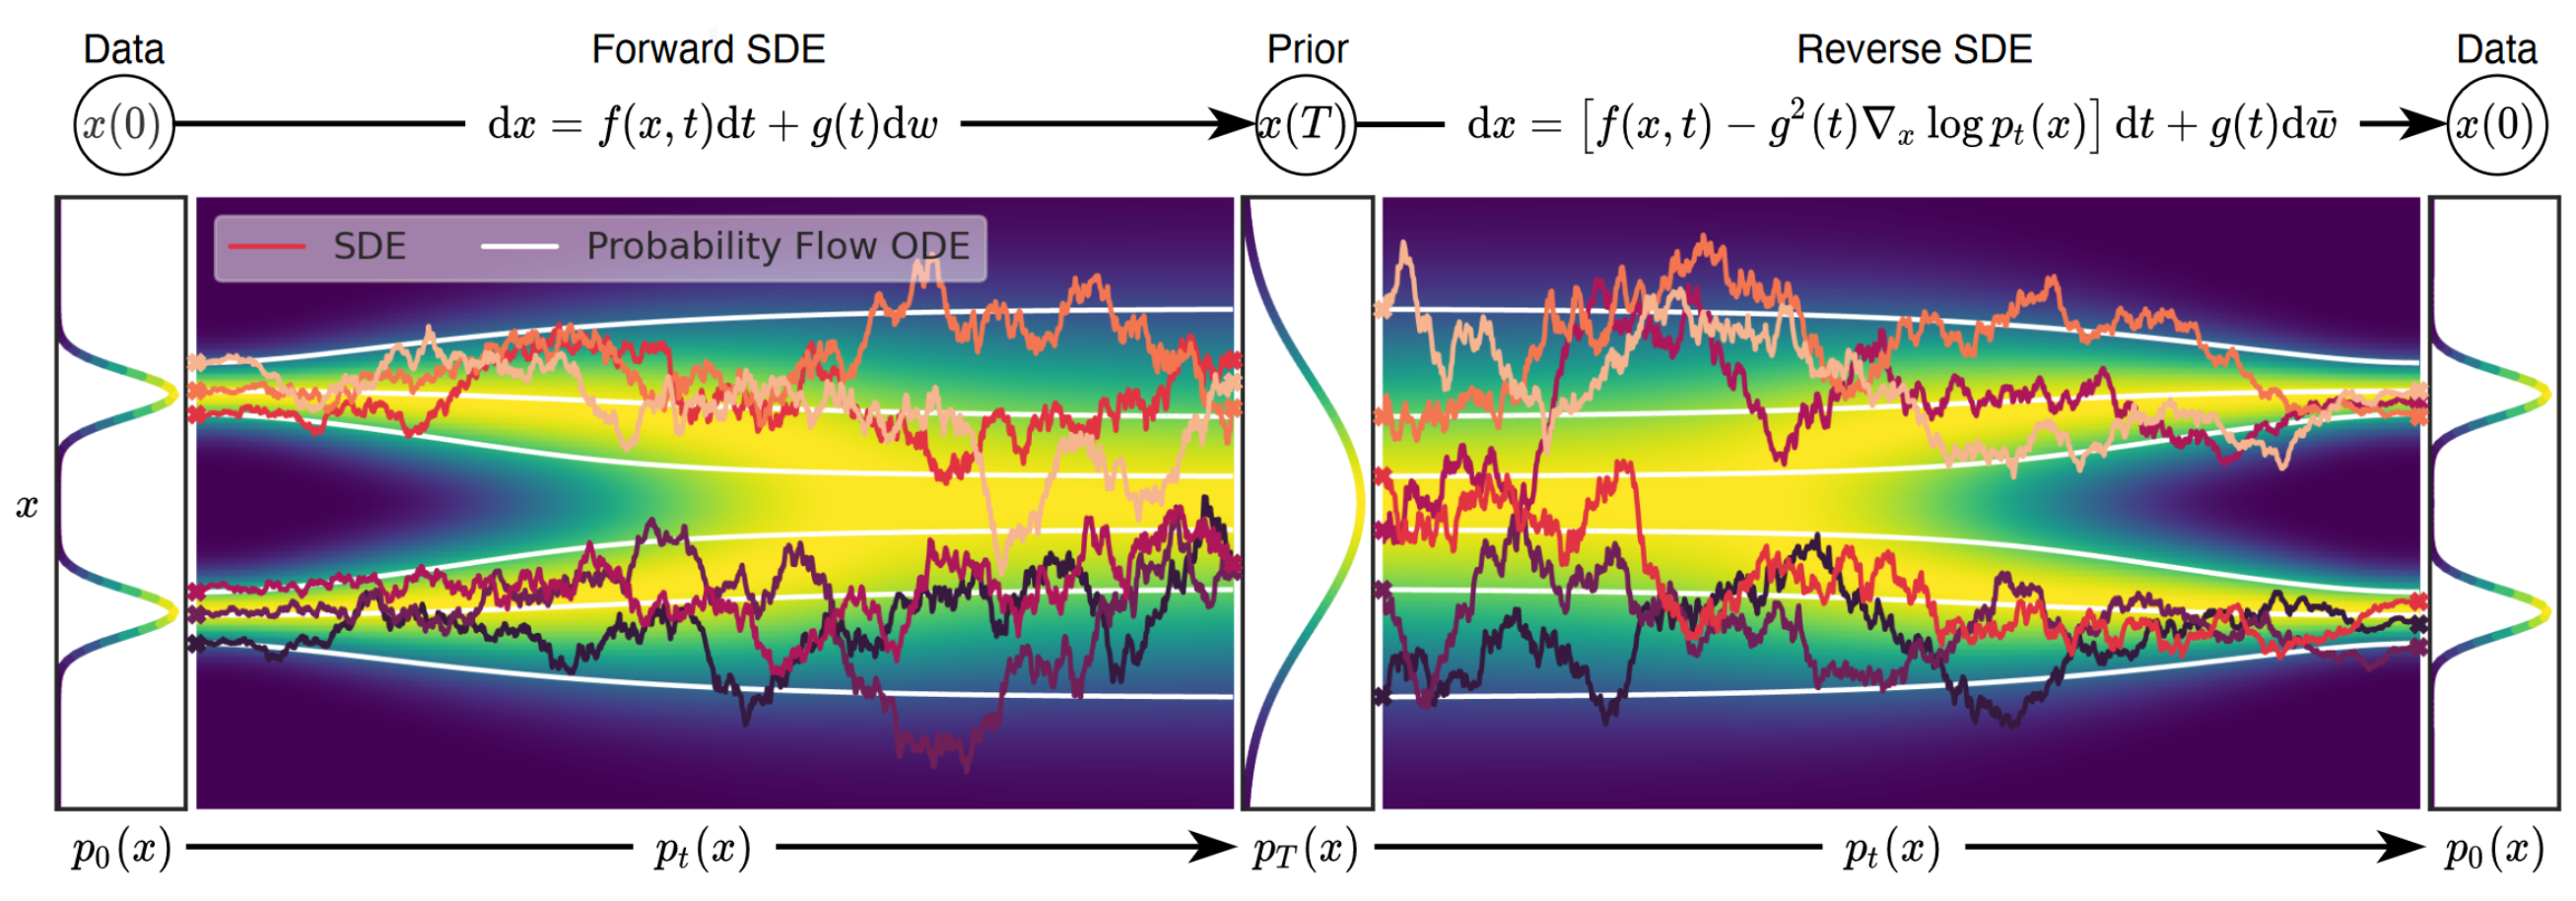
\includegraphics[width=1\columnwidth]{figures/DiffusionModels_SDEs.png}
    \caption{Summary of the score-based generative modeling through SDEs \citep{song2020score}}\label{fig:DM_SDEs}
\end{figure}

Knowledge of the scores at each time requires the estimation of the scores for an SDE which involves training a model to approximate the gradient of the log probability of data at various noise levels \citep{song2020score}. The training objective is given by:

\[
\theta^* = \arg\min_\theta \mathbb{E}_t \left\{ \lambda(t) \mathbb{E}_{x_0} \mathbb{E}_{x_t|x_0} \left\| s_\theta(x_t, t) - \nabla_{x_t} \log p_{0t}(x_t | x_0) \right\|_2^2 \right\}
\]

\citep{song2020score} The equation presents a method to find optimal model parameters \( \theta^* \) that minimize the expected discrepancy between the scores estimated by the model and the actual data transition scores over time, which are influenced by the noise \citep{song2020score}. The expectations are taken over time and modulated by a time-varying weighting function \( \lambda(t) \). ``With sufficient data and model capacity, score matching ensures that the optimal solution for the above equation, denoted by \(s_\theta*(x, t)\) equals \(\nabla_{x_(t)} \log p_{t}(x)\) for almost all \( x \) and \( t \)'' \citep{song2020score}. The score matching process matches the output of the score network with the true gradient of the log-likelihood over the course of the SDE, enabling the generation of realistic data samples from complex distributions \citep{yangdiffusionSummary}.


